%************************************************
\chapter{Introduction}\label{ch:introduction}
%************************************************

CERN, European Organization for Nuclear Research, (French: Conseil européen pour la recherche nucléaire) is an European research organization that operates the largest particle physics laboratory in the world.

Its mission is to:
\begin{itemize}
	\item Provide a unique range of particle accelerator facilities that enable research at the forefront of human knowledge
	\item Perform world-class research in fundamental physics
	\item Unite people from all over the world to push the frontiers of sciences and technology, for the benefits of all.
\end{itemize}

It host the instrument of the 4 biggest physic collaboration: 
\begin{itemize}
\item ALICE
\item ATLAS
\item CMS
\item LHCb
\end{itemize}

CERN host also a plethora of smaller physical collaborations that benefits from the instruments, know how, network effect and services availables.

Between the services offered to its users the computing service is one of the most interesting. Indeed CERN host and manage one of the biggest computing datacenter used for public research.

An issues that affect the operations inside the datacenter is the provisioning of software on the computing servers.

A specialization of the same problem is the provisioning of containers images.

The general problem of software provisioning is been solved by the use of CVMFS, a read only file-system that provides a scalable, reliable and low maintenance software distribution system.

This thesis will explore the problem of creating a suitable read-only file-system structure to provision containers images on computing nodes. We will provide a general read-only filesystem structure and we will implement the proposed methodology on top of CVMFS.

This thesis is composed by several parts:
The background will provide the necessary information on the CERN computing architecture (WLCG), then we will explore CVMFS and why it is a good fit for the CERN computing architecture, the last part of the background will cover the integration between CVMFS and containers technologies.
The state of the art will explore what alternatives are available for software distribution in general and for distribution of images.
We will then define the problem that this thesis is trying to solve and few metrics of interest in our specific case.
The methodology part will explain the details of the solution we propose for this specific problem.
The implementation chapter will focus on how the proposed methodology is been put in practise.
We will evaluate the result of the proposed methodology and implementation on the result part following the metrics that were previously proposed.
Finally we will propose future work and enhancement to the implementation


\section{WLCG}

The Worldwide LHC Computing Grid is an global collaboration of more than 170 datacenters in 42 countries.
The mission of the WLCG is to provide the computing resource to store, distribute and analyze the data from the operation of the LHC.

The organization of the WLCG follow a hierarchical model, where each level is called “Tier”
The most central Tier is the Tier-0 hosted by CERN in the Geneva Area and in Budapest. There are 13 Tier-1 datacenter with enough storage and computing capabilities to support the Grid operation around the clock, the Tier-1 are connected to the Tier-0 with at least 10Gb/sec links. 
Tiers-1 are geographically distributed, 8 of them are in Europe, 3 in the North American and the rest in Asia. Finally the Tier-2 datacenter do not have strict requirements and are generally operated by research centers and universities.

The work on the WLCG is mostly divided in two big classes: analysis of the data from the LHC detectors and Monte Carlo simulations.
The WLCG assume and support a batch computing paradigm. Analysis are splitted in smaller jobs that are distributed to different servers that can work in parallel.

Before to start each job it is necessary to install the software on the server. Unfortunately the amount of software potentially needed in each computing node and the velocity at which the software is updated makes the installation challenging. Moreover simpler installation techniques that relies on packages managers are not applicable since they would put the package managers themselves under too much load.

Several solution have been proposed and used, but eventually it settled for the use of CernVM-FileSystem (CVMFS).

\section{CVMFS}

CernVM-FileSystem provides a scalable, reliable and low-maintenance software distribution system. It is implemented as a read-only POSIX file-system in user space exploiting FUSE (Filesystem in USErspace) and standard webserver technologies such as Apache or NGNIX.

CVMFS organize its content in repositories where we can approximate each repository as a CVMFS instance.

CVMFS is engineered to support repository of size on the order of the Terabyte with billions of files.

To save space files are addressed by their content (Content Addressable Storage), hence duplicated files will be stored only once.

In order to distribute software to geographically distant datacenters and keep a low latency, CVMFS allows to cache content in different machines. This allow to host a cache server in each Tier of the WLCG. The use of caches fits perfectly with the Tiers models of the WLCG presented above. The Tier-0 host the main repository (Stratum-0), and the Tier-1 host the first level of cache (Stratum-1) and so on.

The content of the files are served using the HTTP protocol by a standard webserver. The files are lazily downloaded only on the machine that need them and only when necessary.

In order to locate and request files from CVMFS the clients download the catalog a simple SQLite database which describes a subtree of the whole filesystem.
The catalog contains all the metadata of files and directories, including owner, group, permission, and size. Moreover the catalog contains also the URL where to download the files.

A root catalog is available in a know path, and, if the filesystem grows too large, the root catalog links to other sub-catalogs. The use of sub-catalogs allows to keep each catalog small improving the query time.

\section{Containers}

While CERN solved its problems of software distribution with CVMFS the industry opted for a different approach, containers.

Containers are a standard unit of software that packages up code and all its dependencies so that computer applications run quickly and reliable from one computing environment to the others.

There are two implementation of containers technology widely used at CERN: Singularity and Docker.

\subsection{Singularity}

Singularity focus on running computation on HPC clusters, its main advantage is to be able to run a containers from a standard directory. It is sufficient that all the content of the containers is unpacked on a single directory to run the container itself using Singularity. Finally, Singularity does not rely on a daemon running in the host machine unlike docker.

Singularity is able to run specific Singularity images as well as more generic Docker images.

Given the capability of Singularity to bootstrap the containers from a simple directory the integration with CVMFS is straightforward: create on CVMFS a directory for each kind of Singularity container we wish to run. The Singularity software will read those directories and run the correct container.

\subsection{Docker}
\label{subsec:docker-thin-images}

Docker is more widespread in the industry and benefits from more mature tools and ecosystem, however docker needs root permissions in order to run a container and a background daemon (dockerd.) Moreover the filesystem of docker containers is encapsulated inside the docker daemon which needs to download it from an external sources, uncompress it, cache it, and mount it. 

Given the advantages and widespreads of containers they started to be used also inside CERN and integration with the CERN existing software distribution infrastructure (CVMFS) was required. 
Without the integration with CVMFS, to run a container it is necessary to download all the container content on the machine, while it has been showed that, on average, only 7\% of the content of containers is actually needed. 
The integration would allow to download only the strict necessary files.

The integration with docker was more complex. In this work we are not concerned about the implementation details of the integration between docker and CVMFS, but we are concerned with the interface of such integration.

It is not possible to host docker layers on CVMFS and use them directly. The solution was to create a new kind of images, called “Thin-images”.
Thin-images consist in only a file, the “recipe”, that describe the content of the original image in terms of layers.
The recipe file is then read by a docker plugin. The plugin makes the content of the original image available to the docker daemon through CVMFS. This procedure allows to run docker images without the need to download all the files in the image itself.
The creation of a thin-images consist in making the several layer of the original docker images available in CVMFS, create the “recipe” file which contains the location of all those layers, and finally create a docker image that contains only the “recipe” file.

\begin{figure}
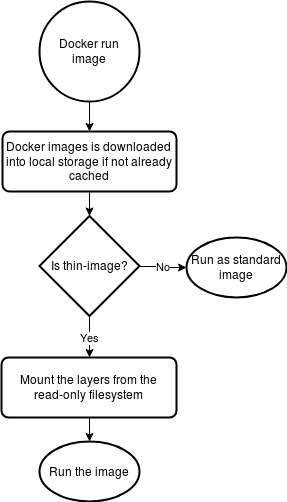
\includegraphics{gfx/RunThinImages}
\label{fig:flowchart-run-thin-image}
\caption{Decision proces for running docker thin images}
\end{figure}

\subsection{Containers distribution}
\label{subsec:singularity-docker-distribution}

Containers can be distributed to the host in several ways, in this works we are mostly concern with the simplest alternative, the use of registries and, specifically, the use of docker registries.

The content of a container is packed in “layer”, each layer stores the “delta” between a computing environment and the other, an "image" is an immutable set of layers. Containers are an instances of images.

Each layer is identify by its digest. The whole content of the layers is hashed (generaly using the hash256 function) and the result of the hash function is the digest of the layer.

The same schema is adopted for images as well, indeed, each image is identifies by the digest which is the hash of all its content.

The layers are distributed, generally, over the network as compressed tar archives that need to be downloaded, then uncompressed and potentially cached.

The components responsible for distributing the layers are the registries. The registries expose an HTTP interfaces that serve the required layer as compressed tar archive.

Docker images are served by docker registries. Moreover, since Singularity can run Docker images, one of the most common way to share Singularity images is to make them available as normal docker images into standard docker registries. 

At runtime layers are composed one on top of each other to re-create the original environment where to execute the application.

This approach to container distribution is standardize in the OCI standard.

While containers ensures a complete reproducibility of the environment every files in every layer need to be present in the hosting machines, i.e. in the machine running the application.


